\chapter{Sprint 1: Authentication and User management}



\section*{Introduction}

\addcontentsline{toc}{section}{Introduction}

Considering the product backlog, and having planned the execution of the project for a course of three sprints, we focus on the first sprint. The sprint aims at setting up the skeleton of the project and the implementation of safe authentication and user management.

\section{Sprint Backlog}
To start, we outline the work to be done in this sprint. The schedule for this iteration
involves the user stories described in the following Table 3.1:

\begin{longtable}{|l|p{6cm}|p{8cm}|}
\hline
Sprint & User story & Task\\
\hline
\multicolumn{3}{|c|}{Initializing the project structure} \\
\hline
\endfirsthead

\multicolumn{3}{c}{{\bfseries}} \\
\hline
Sprint & User story & Task\\
\hline
\endhead

\hline \multicolumn{3}{|r|}{{Continued on next page}} \\ \hline
\endfoot

\hline
\endlastfoot

1 & As a student, I want to register easily and securely & \begin{itemize}
    \item Create the user model
    \item Create user registering feature on the server-side
    \item Create user registering interfaces
    \item Integration and testing
\end{itemize} \\ \hline

2 & As a student, I want to log in to a space reserved for students & \begin{itemize}
    \item Create login feature using web tokens
    \item Create user login interfaces
    \item Integration and testing
\end{itemize} \\ \hline

20 & As a student, I want to manage my account & \begin{itemize}
    \item Create user profile management features on the server side
    \item Create profile management interfaces
    \item Integration and testing
\end{itemize} \\ \hline

6 & As a student, I want to receive an email to change my password if I have forgotten it & \begin{itemize}
    \item Integrate emailing feature in server-side using Node Mailer
    \item Create forget password Interfaces
    \item Integration and testing
\end{itemize} \\ \hline

11 & As a student, I want to change my password & \begin{itemize}
    \item Create changing password feature in the backend
    \item Create changing password interfaces
    \item Integration and testing
\end{itemize} \\ \hline

5 & As a student, I want to receive an email to activate my account & \begin{itemize}
    \item Create user account activation features on the server side
    \item Create account activation interfaces
    \item Integration and testing
\end{itemize} \\ \hline
\caption{Sprint 1 backlog}
\label{Tab: Sprint 1 backlog}
\end{longtable}


\section{ Analysis and conception}
In this section, we illustrate the sprint analysis in a more visual representation using use case diagrams and sequence diagrams of the most highlighted features:
"Login" and "Signup".

\subsection{Use case diagrams}
More detail on the “login” use case can be found in figure 3.1 that rounds up the diagram of the use case.

\begin{figure}[H] 
            \centering
            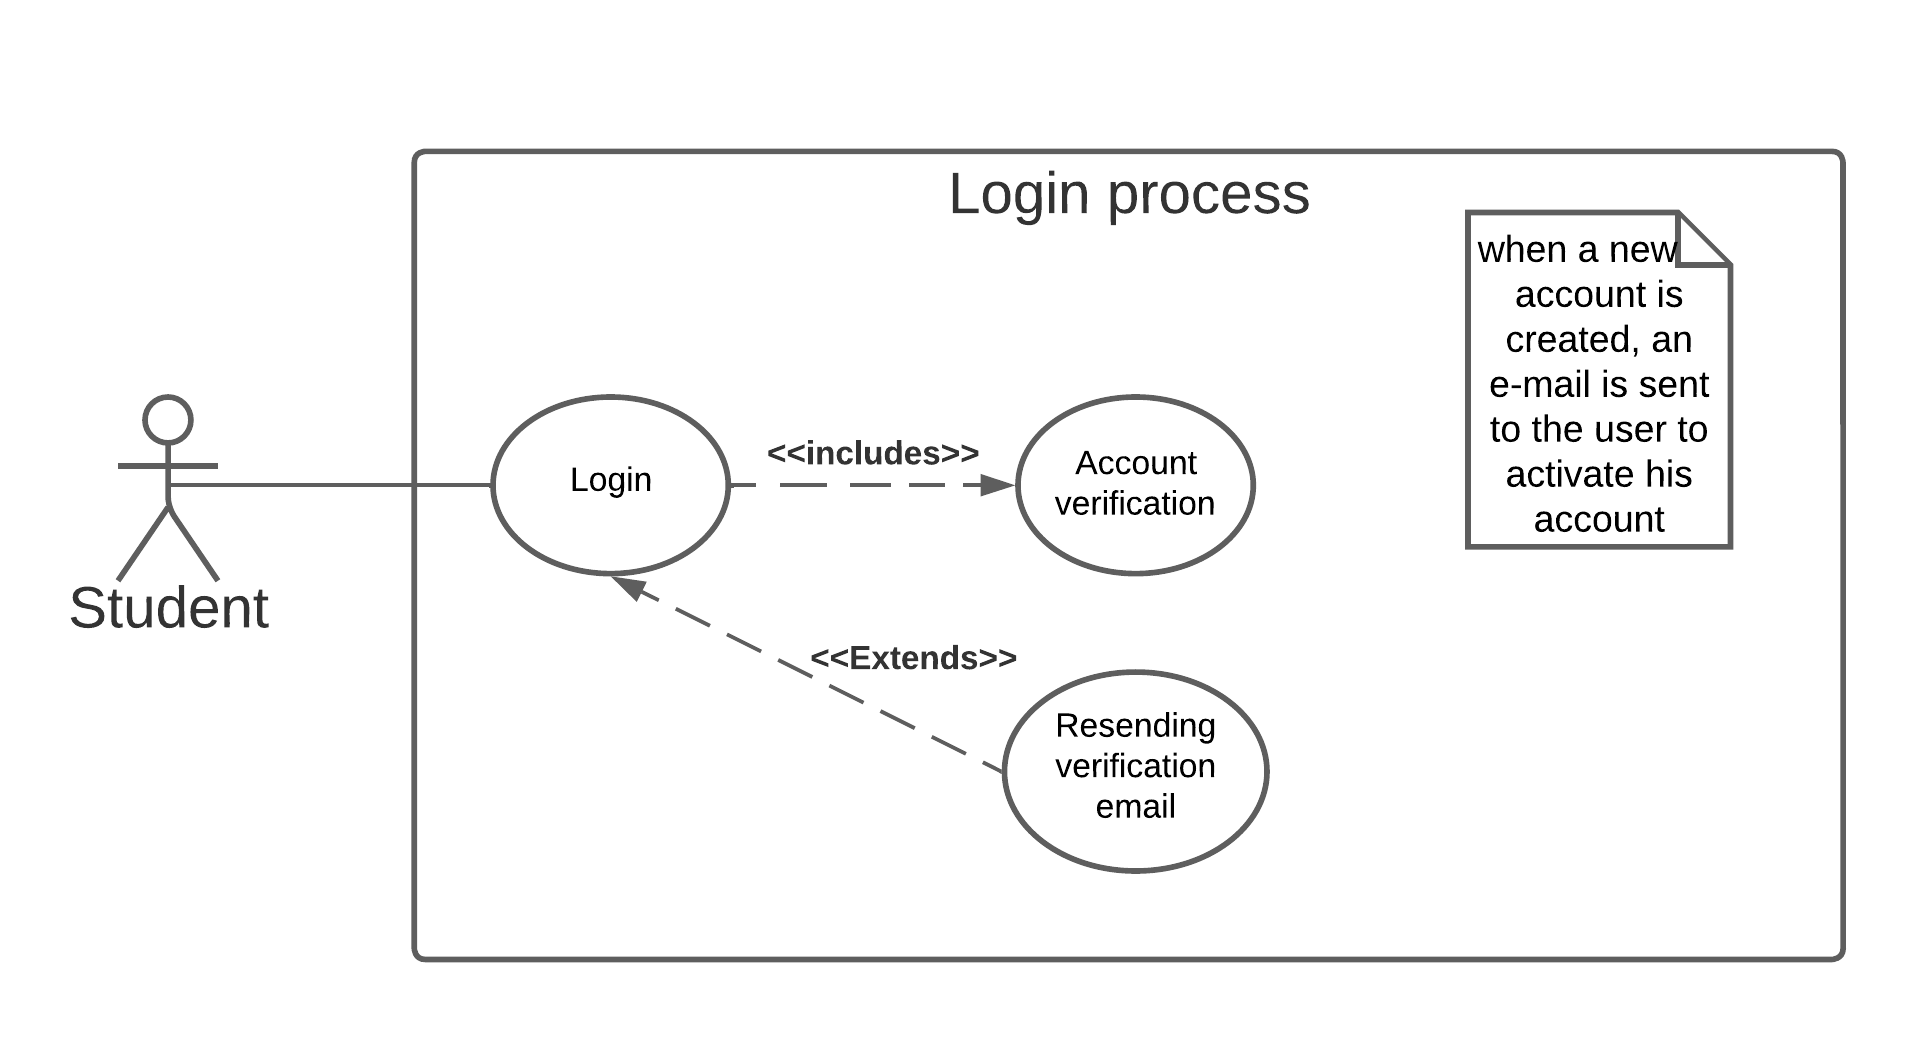
\includegraphics[scale=0.9]{diagrams/refined use case login.png}
            \caption{Login use case diagram} 
            \label{fig: Login use case diagram}
\end{figure}

The diagram of the "Signup" use case is shown in figure 3.2 :

\begin{figure}[H] 
            \centering
            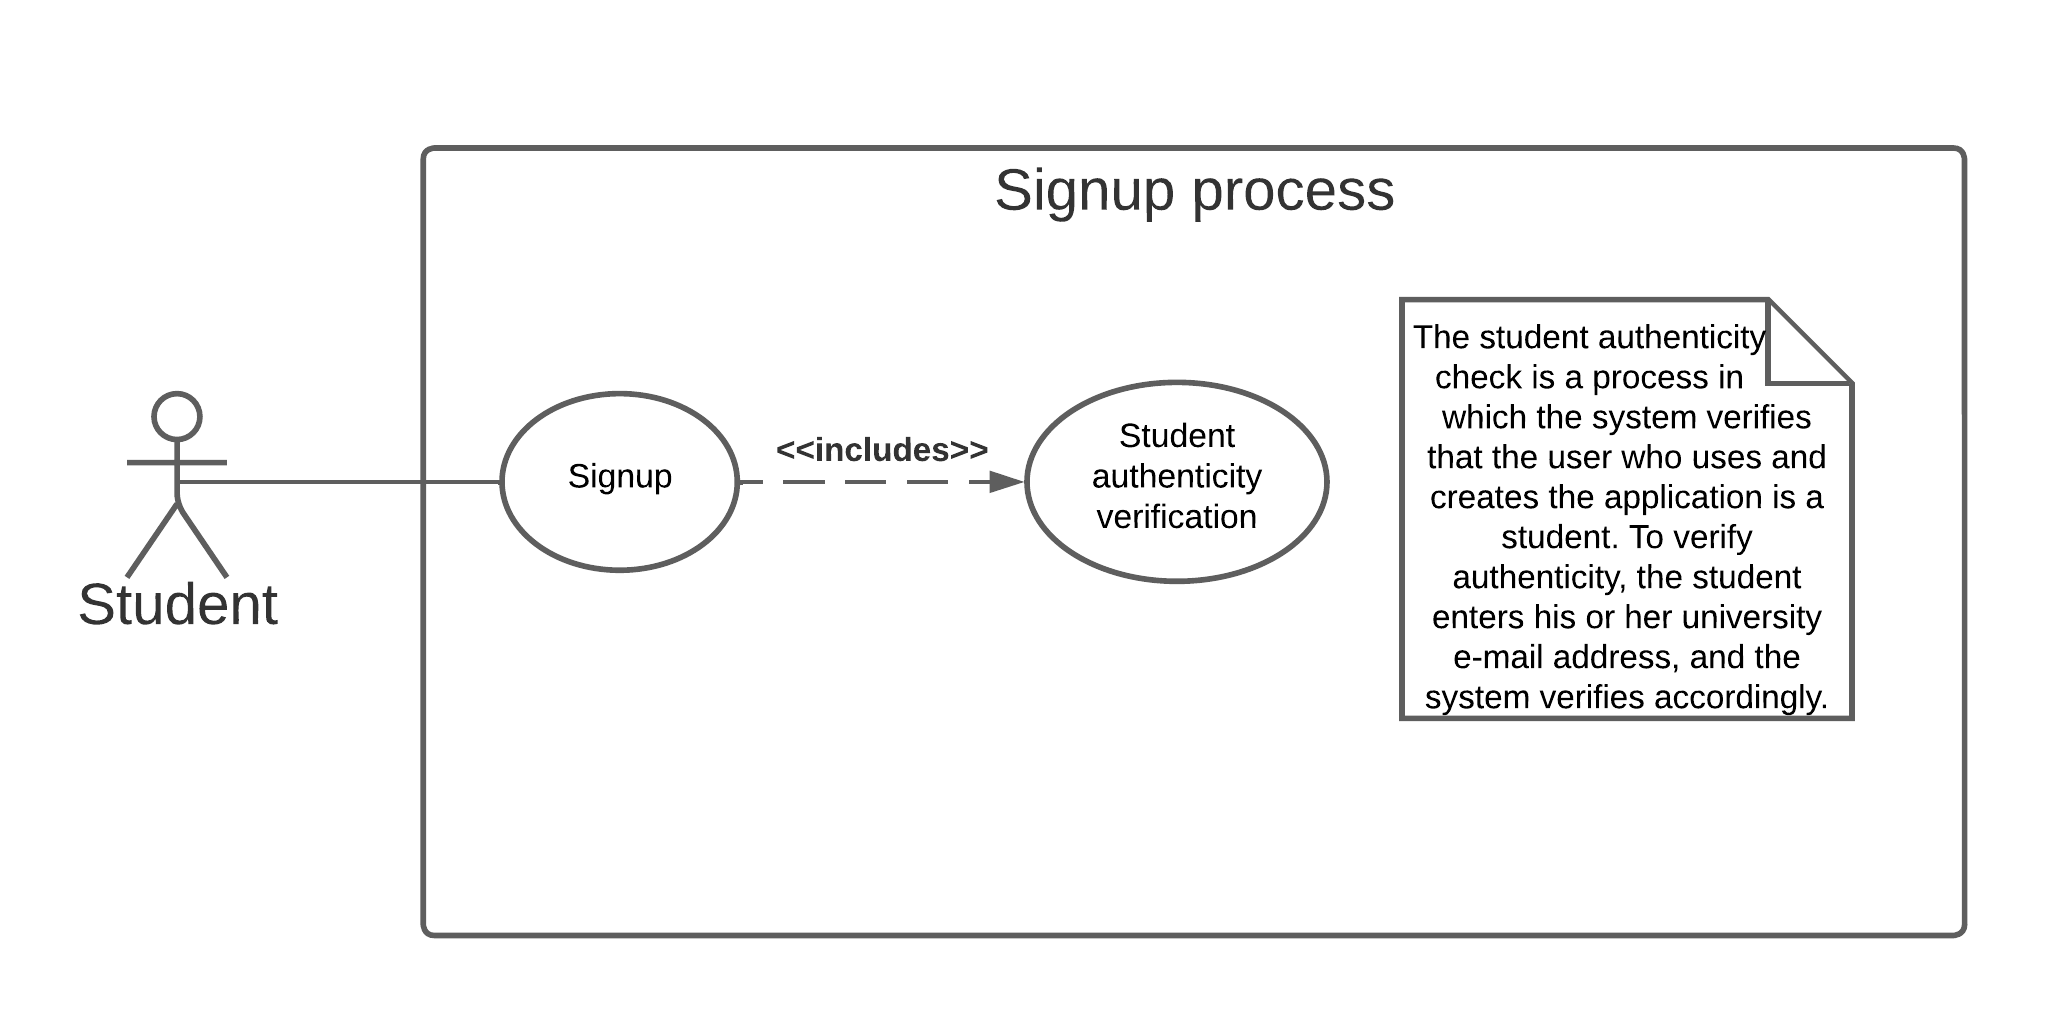
\includegraphics[scale=0.9]{diagrams/refined use case signup.png}
            \caption{signup use case diagram} 
            \label{fig: signup use case diagram}
\end{figure}

\subsection{Use case textual descriptions}
Textual descriptions of the "Login" use case are illustrated in table 3.2 below:
\begin{longtable}{|c|p{10cm}|}
\hline
Use Case & Description \\\hline
Name & Login use case \\\hline
Preconditions & The student's account must be active \\\hline
Postconditions & The student is logged in to a student-only space \\ \hline
Main Flow & \begin{enumerate}
    \item The user puts his coordinates(email and password) 
    \item The system checks if the account is activated or not
    \begin{enumerate}
        \item if the account is activated the user login successfully 
        \item if the account is not activated, the system shows an error message
    \end{enumerate}    
\end{enumerate}
\\\hline
Alternative Flows & \begin{itemize}
    \item if the user is not found, an error message appears
    \item if the user wrote bad credentials, an error message appears
    \item if there is a network error, an error message appears
\end{itemize}
\\\hline
Non-functional Requirements & \begin{itemize}
    \item The login will be secured thanks to the JSON Web tokens
    \item The login will be easy and the user will be aware of any problems
\end{itemize}
\\\hline
\caption{Textual descriptions of the Login use case}
\label{Tab: Textual descriptions of the Login use case}
\end{longtable}

The use case textual descriptions of "Signup" is illustrated in the
following Table 3.3:

\begin{longtable}{|c|p{10cm}|}
\hline
Use Case & Description \\\hline
Name & Signup use case \\\hline
Preconditions & The user must be a student \\\hline
Postconditions & A new account is created and an activation email is sent \\ \hline
Main Flow & \begin{enumerate}
    \item The user puts his university and email so the system can determine if he's a student of that university or not
    \item The user puts his additional information(name , last name , birthday , ...) 
    \item The user puts his pictures and they must be authentic 
    \begin{enumerate}
        \item if one of the information is unacceptable or empty the system shows an error message
        \item if the provided information is acceptable, the account will be created
    \end{enumerate}    
\end{enumerate}
\\\hline
Alternative Flows & \begin{itemize}
    \item if the user is not found, an error message appears
    \item if the user wrote bad credentials, an error message appears
    \item if there is a network error, an error message appears
\end{itemize}
\\\hline
Non-functional Requirements & \begin{itemize}
    \item The login will be secured thanks to the JSON Web tokens
    \item The login will be easy and the user will be aware of any problems
\end{itemize}
\\\hline
\caption{Textual descriptions of the Signup use case}
\label{Tab: Textual descriptions of the Signup use case}
\end{longtable}

\subsection{Sequences diagram}
The login sequence diagram can be observed in Figure 3.3 below:

\begin{figure}[H] 
            \centering
            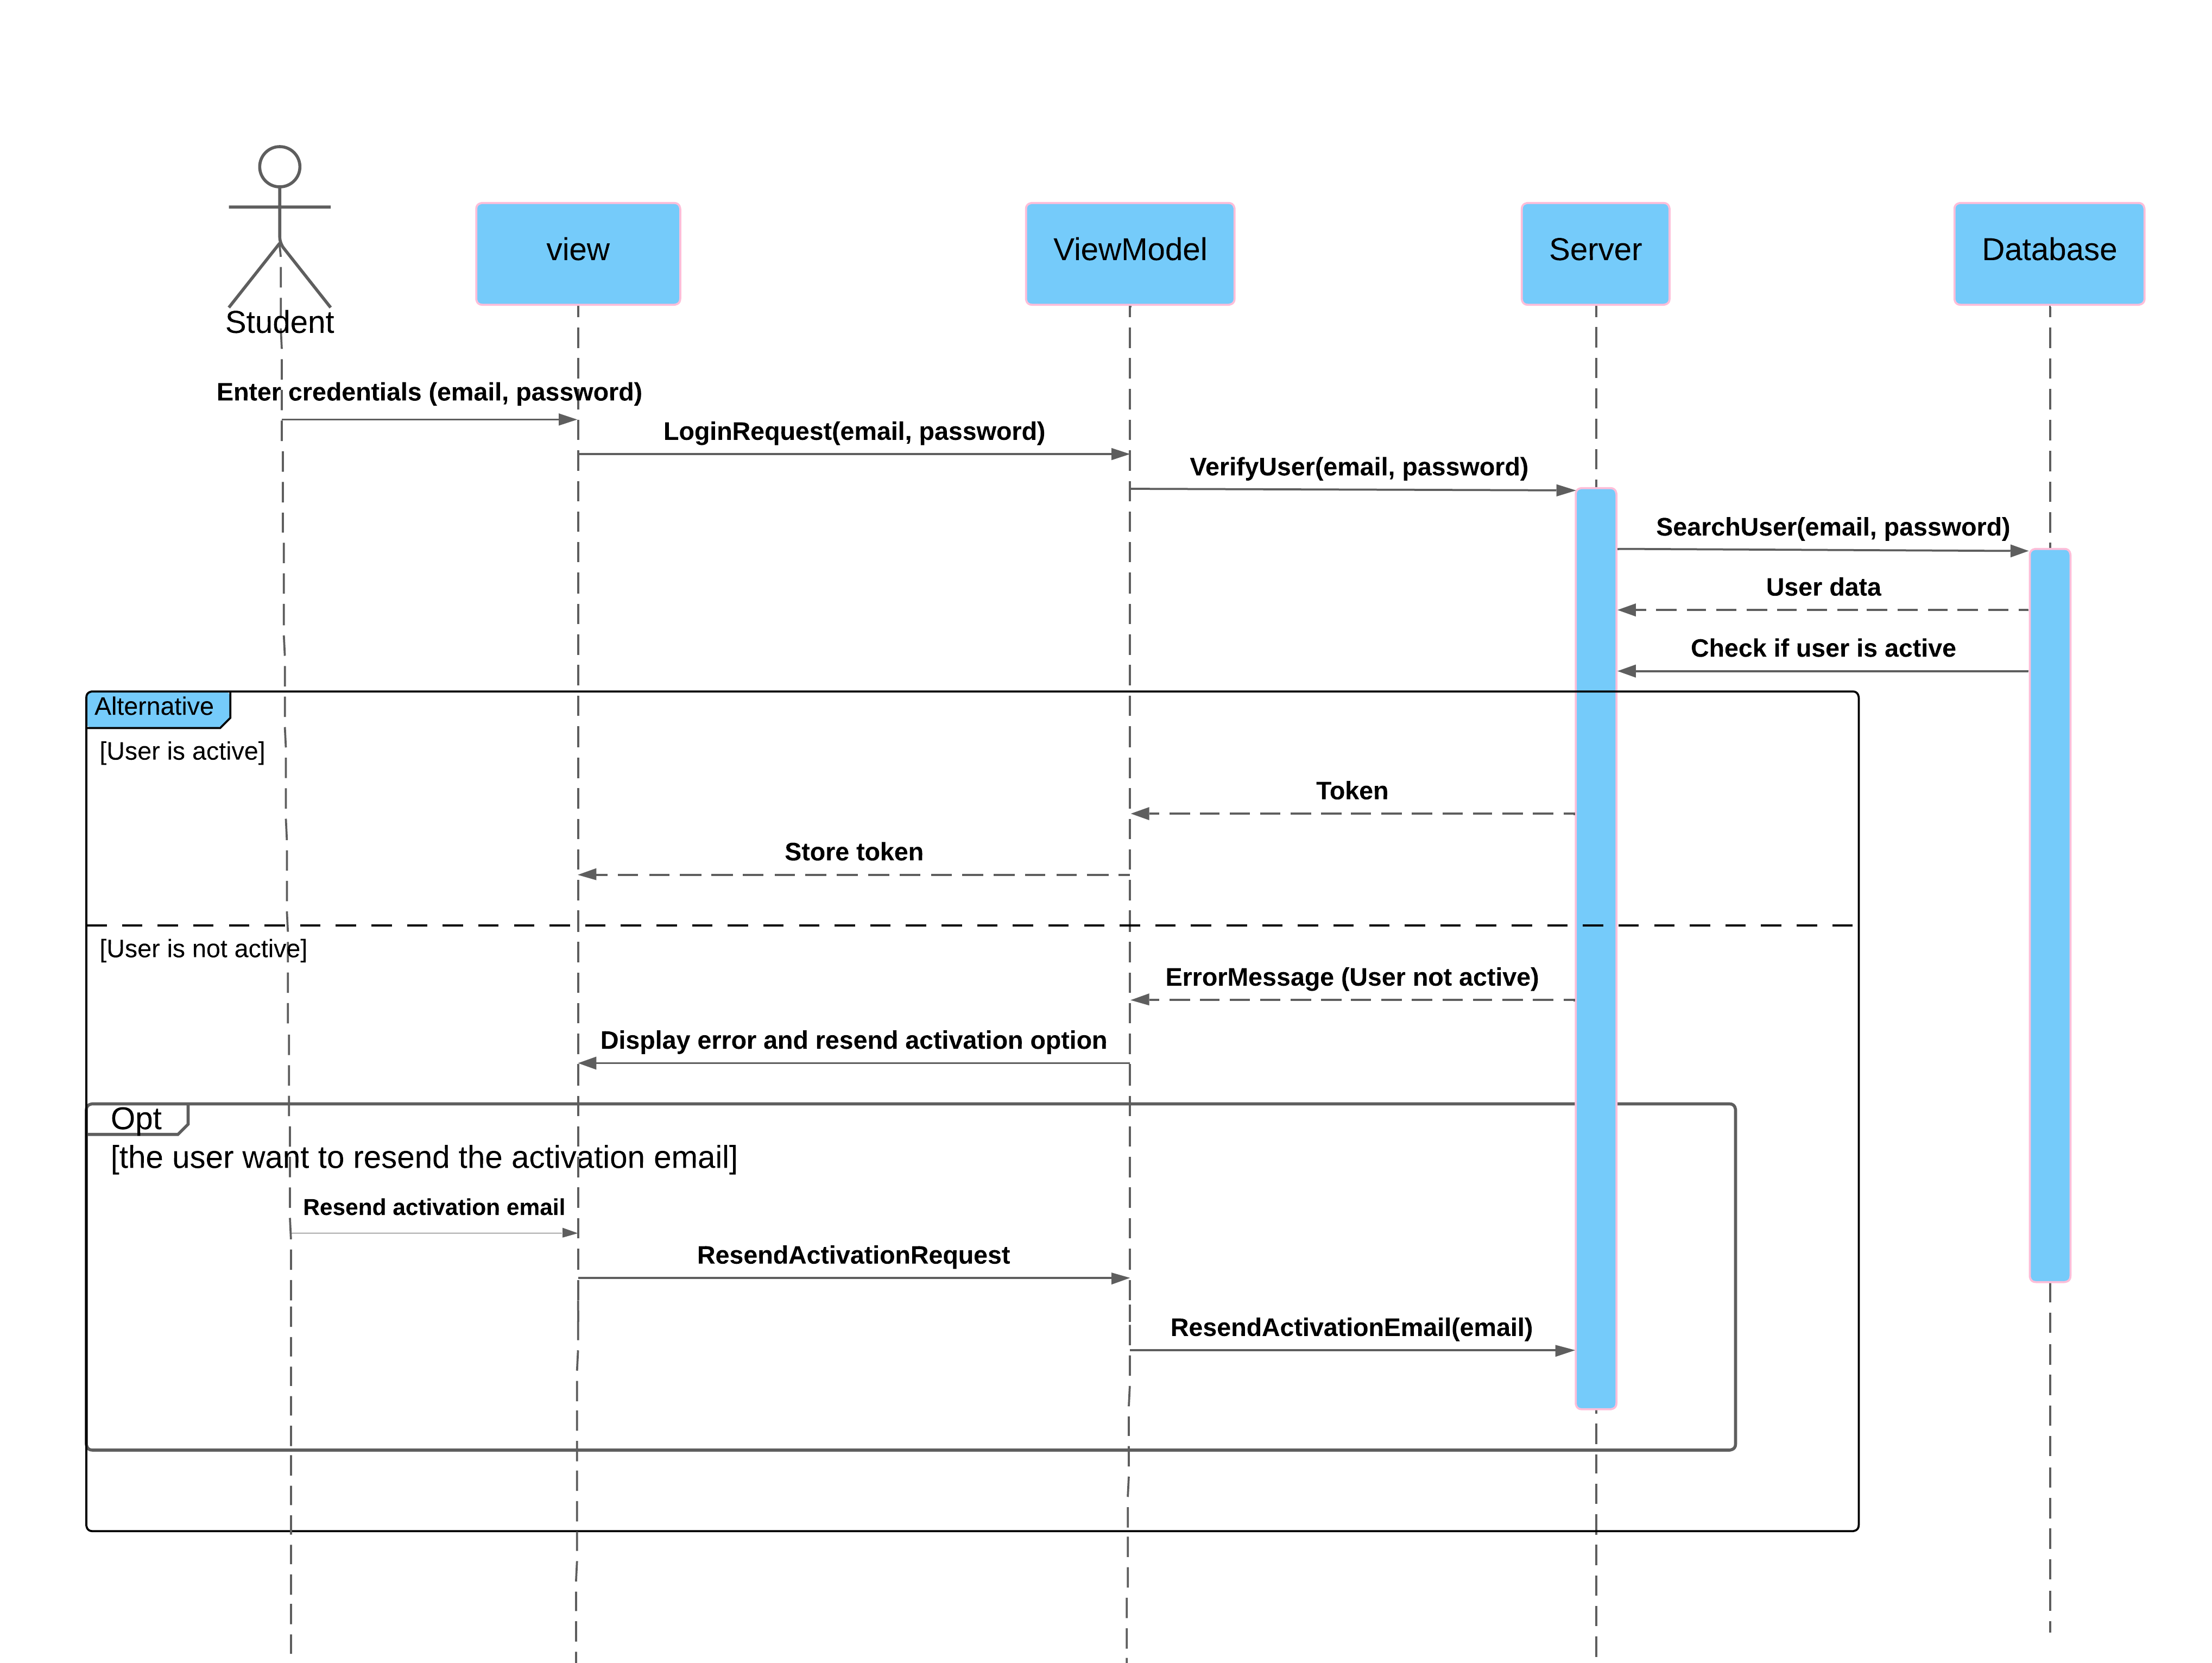
\includegraphics[scale=0.4]{diagrams/object seq diagram login.png}
            \caption{Login object sequence diagram} 
            \label{fig: Login object sequence diagram}
\end{figure}

The Signup system sequence diagram can be observed in Figure 3.4 below:

\begin{figure}[H] 
            \centering
            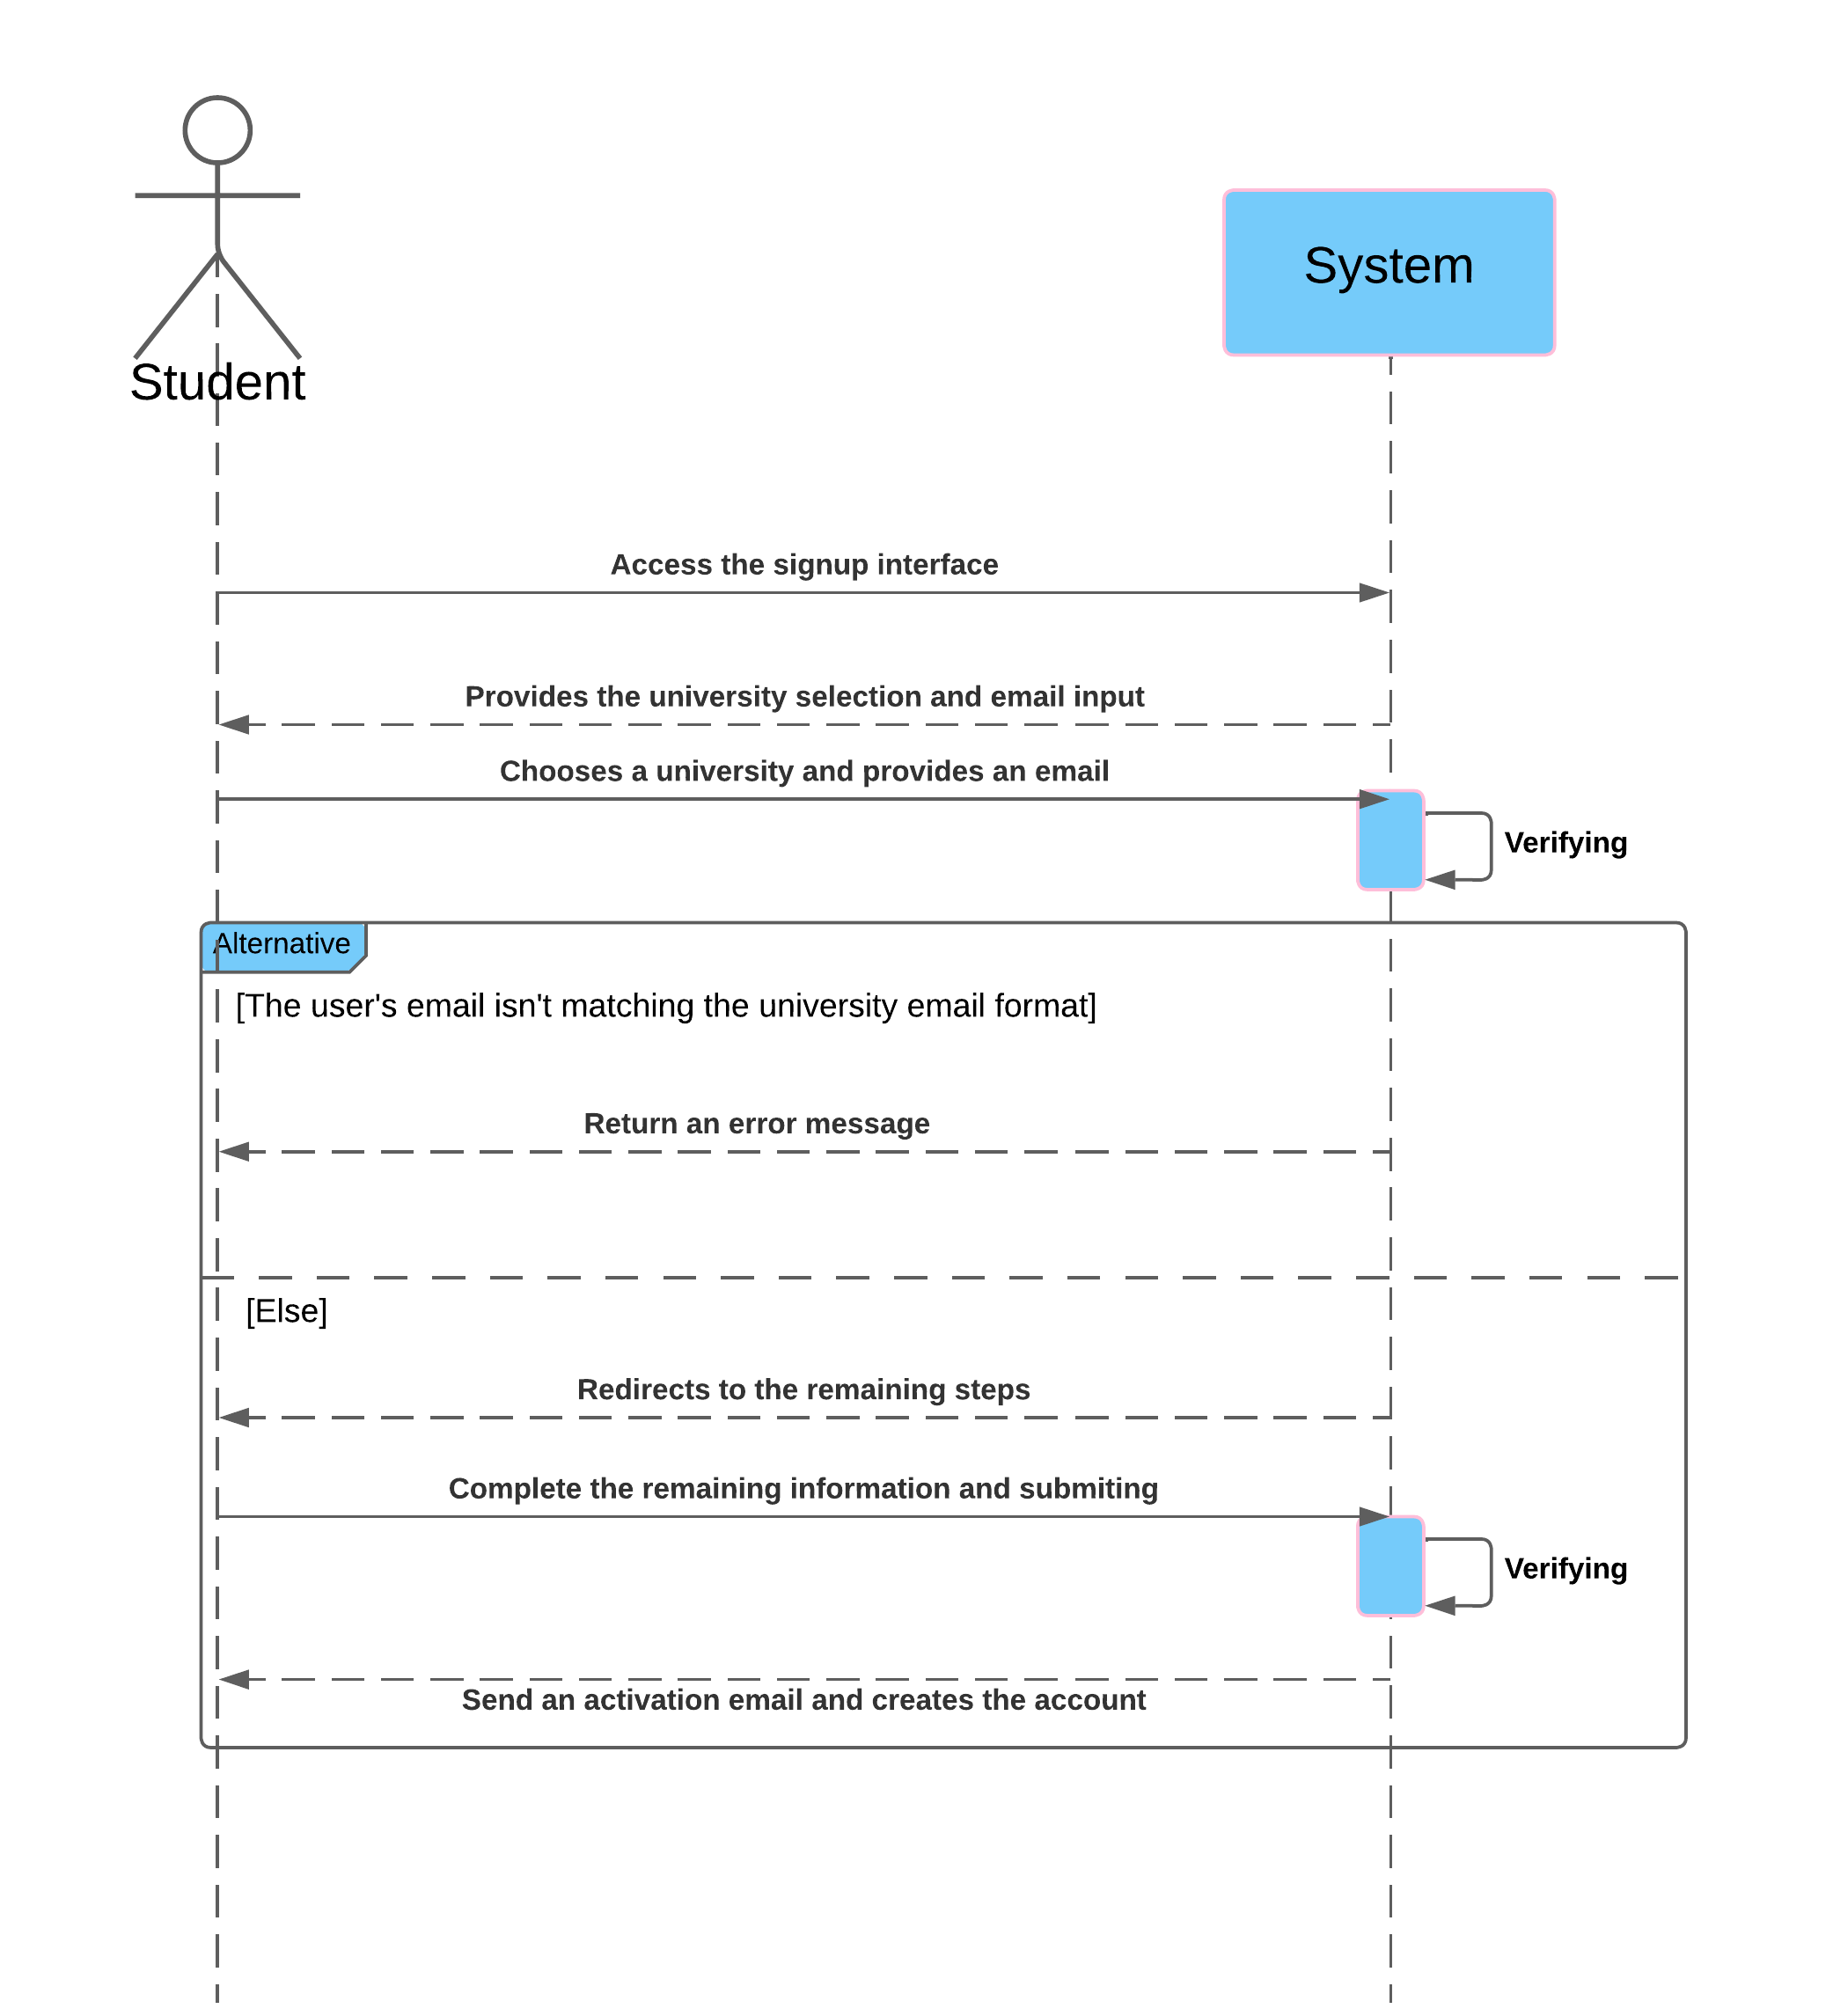
\includegraphics[scale=0.5]{diagrams/system seq diagram signup.png}
            \caption{Signup system sequence diagram} 
            \label{fig: Signup system sequence diagram}
\end{figure}

\section{Realization}
In this section, we describe what has been implemented and how the various components and functionalities identified in this Sprint have been instantiated.

\subsection{User sign-in and registration}
After taking users' needs into account, we created an easy and secure registration method. since the application is for use only by students, how did we manage to give access to the application only to students?
The company's strategy is to open access to the application every university at a time. This enables the company to collect information about the university that will be useful for the verification process. One of many verification processes is to compare the e-mail address provided by the user with the e-mail address format of the selected university using RegEx and check whether or not they match.
Once verified, the student will complete their other data and put on their face to give students an authentic experience and avoid scams and fake profiles thanks to face detection. \\

Below, we take a look at the different stages of the registration process. \\
\begin{figure}[H] 
            \centering
            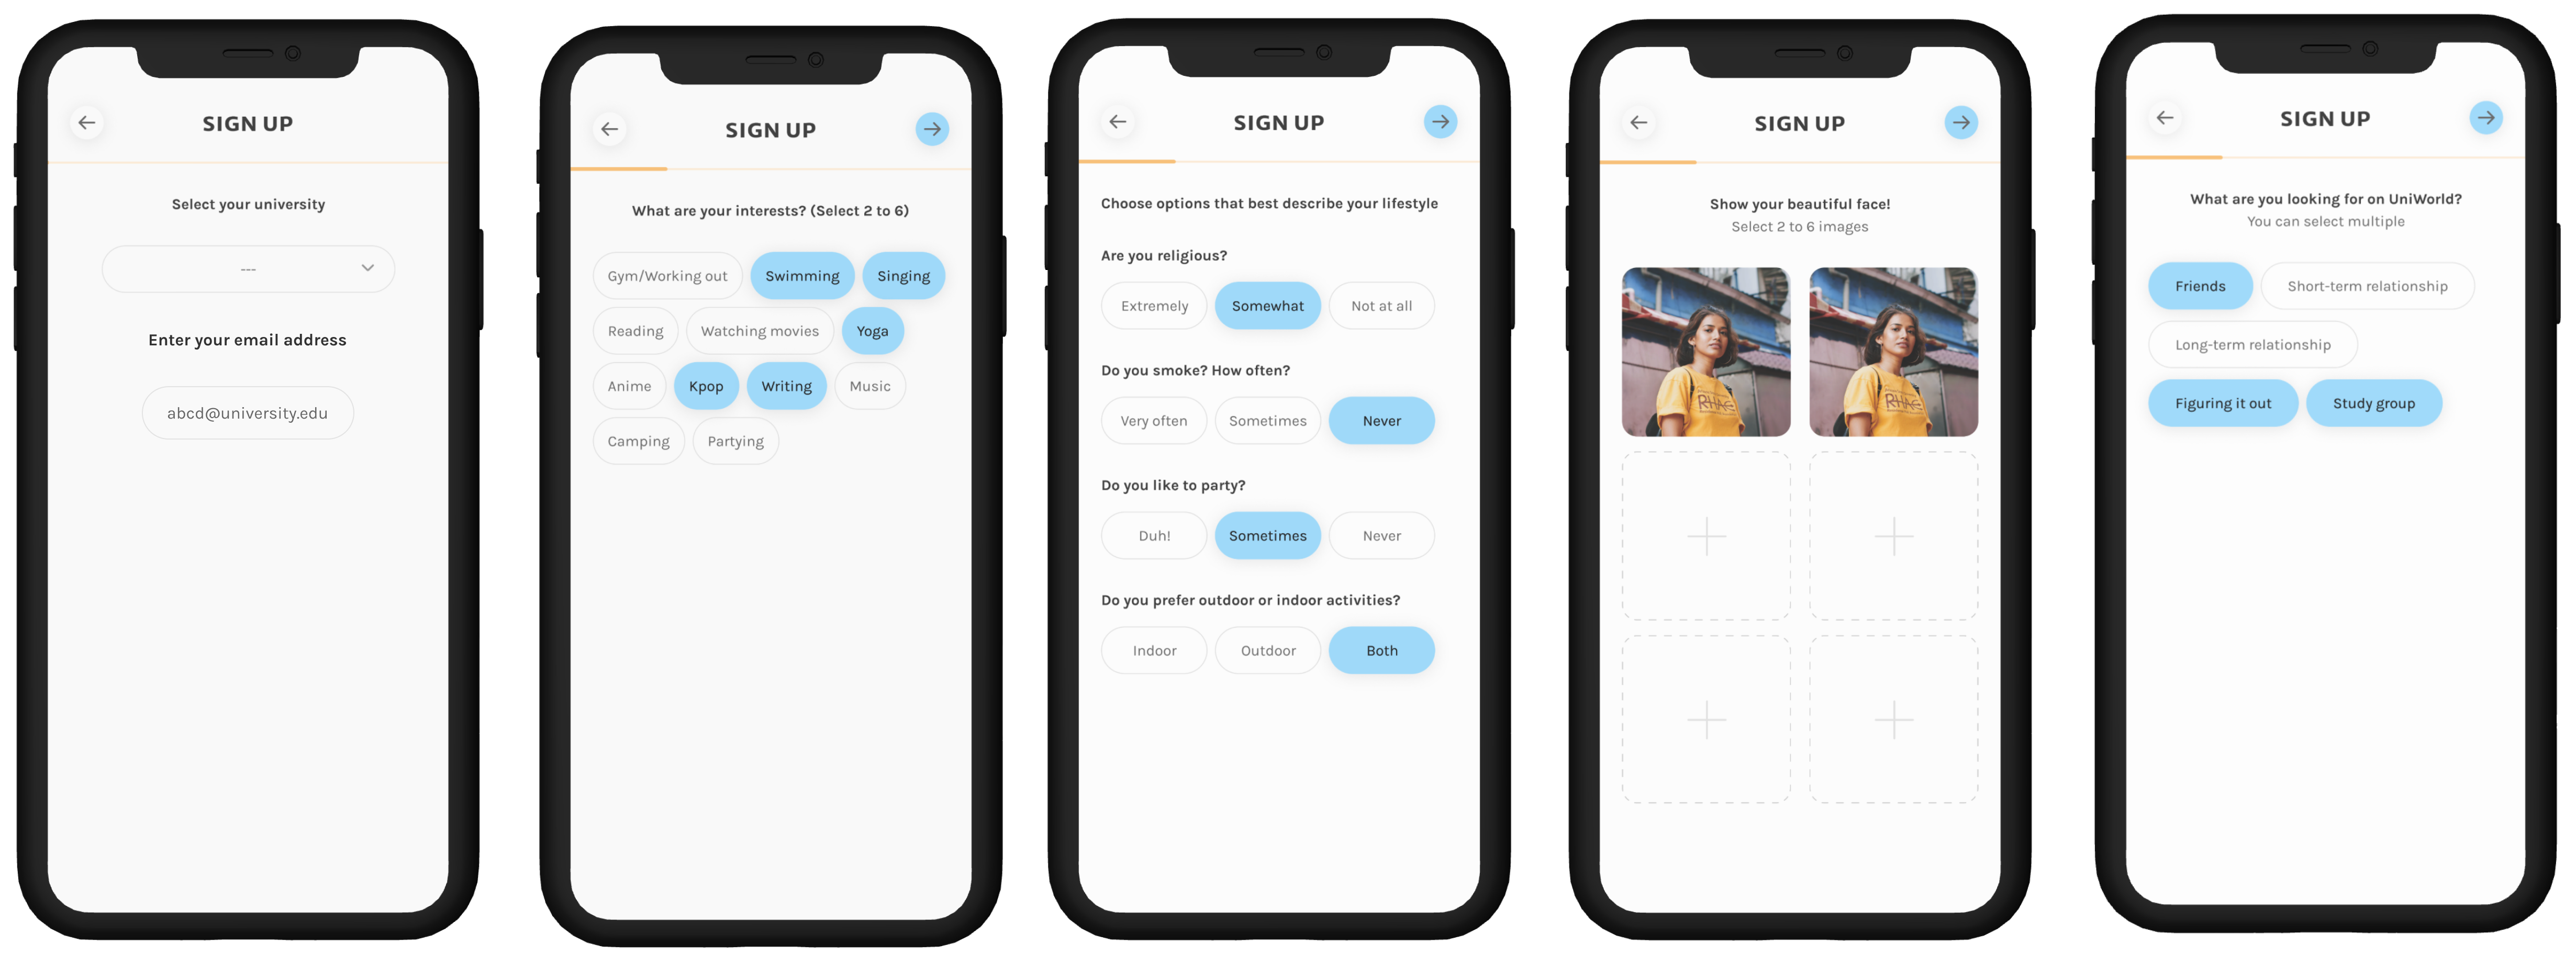
\includegraphics[scale=0.15]{steps signup.png}
            \caption{Some signup steps UI} 
            \label{fig: Some signup steps UI}
\end{figure}
Creating a new account involves hashing the password given by the user, After that it sends a verification mail to the user to activate the account in order to prevent the creation of emails with fake or non-existent emails After the creation of a new account, the login process is relatively simple but optimized for security, the use of JWT for session control has brought unbelievable results in the control of authentication. After activation of the account,  the user inputs his credentials then the system checks whether the user exists and whether his/ her credentials are correct. Once this has been verified, the backend issues out a token to the application and saves it before it is used as a means to authenticate the application’s services. 
The following figure shows the login UI
\begin{figure}[H] 
            \centering
            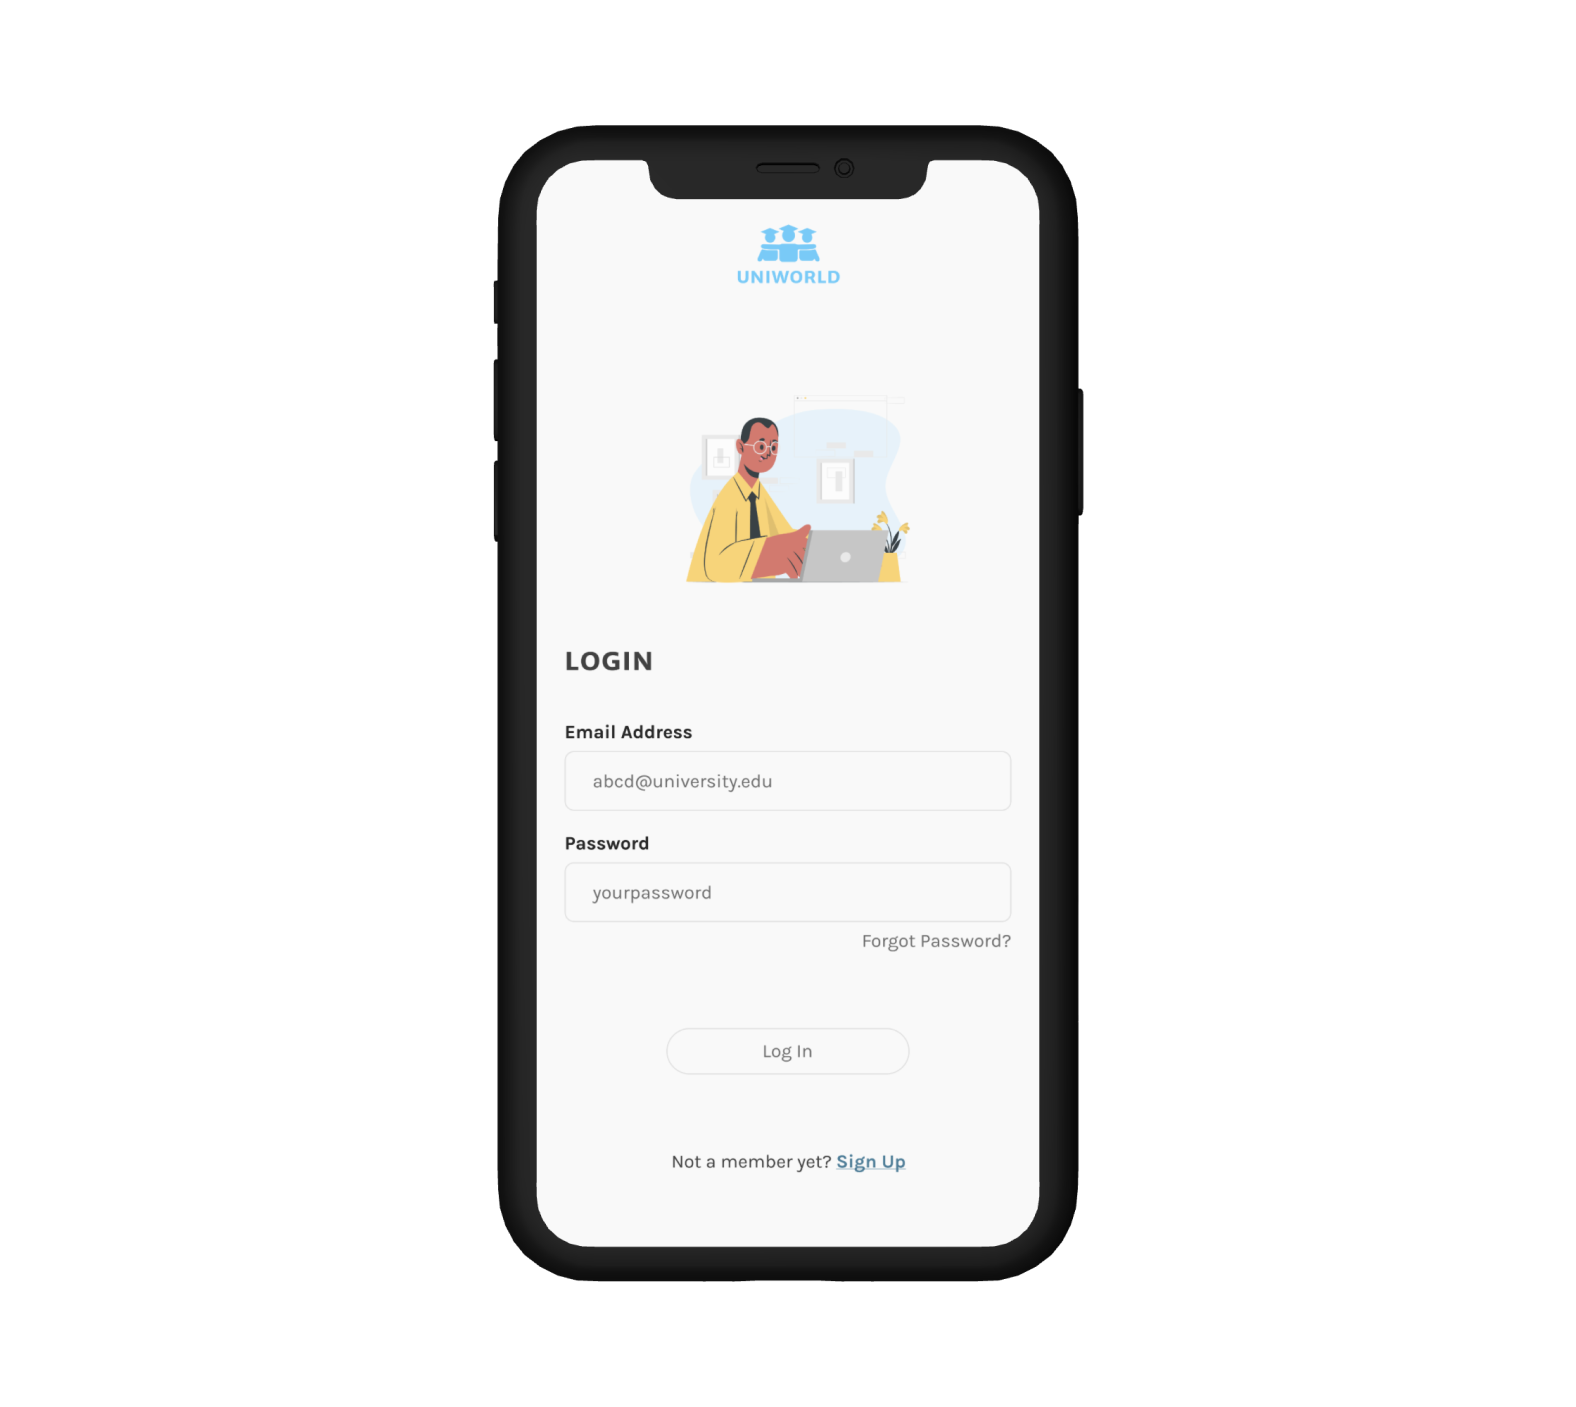
\includegraphics[scale=0.2]{login UI.png}
            \caption{Login UI} 
            \label{fig: Login UI}
\end{figure}
\begin{figure}[H] 
            \centering
            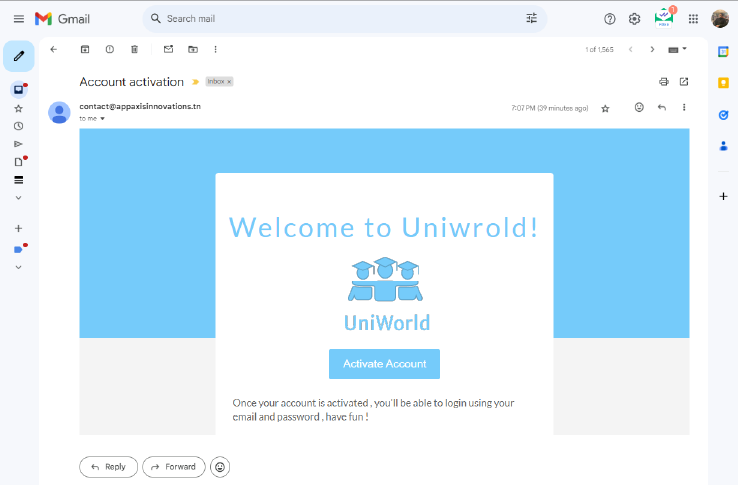
\includegraphics[scale=0.5]{account actiavation mail.png}
            \caption{account activation email} 
            \label{fig: account activation email}
\end{figure}
\subsection{Account management}
After creating an account and logging in, users can manage their account and modify some of the information they have already provided. But first, the system needs the user's token so that he can modify his information.
The account management interface is shown below. 
\begin{figure}[H] 
            \centering
            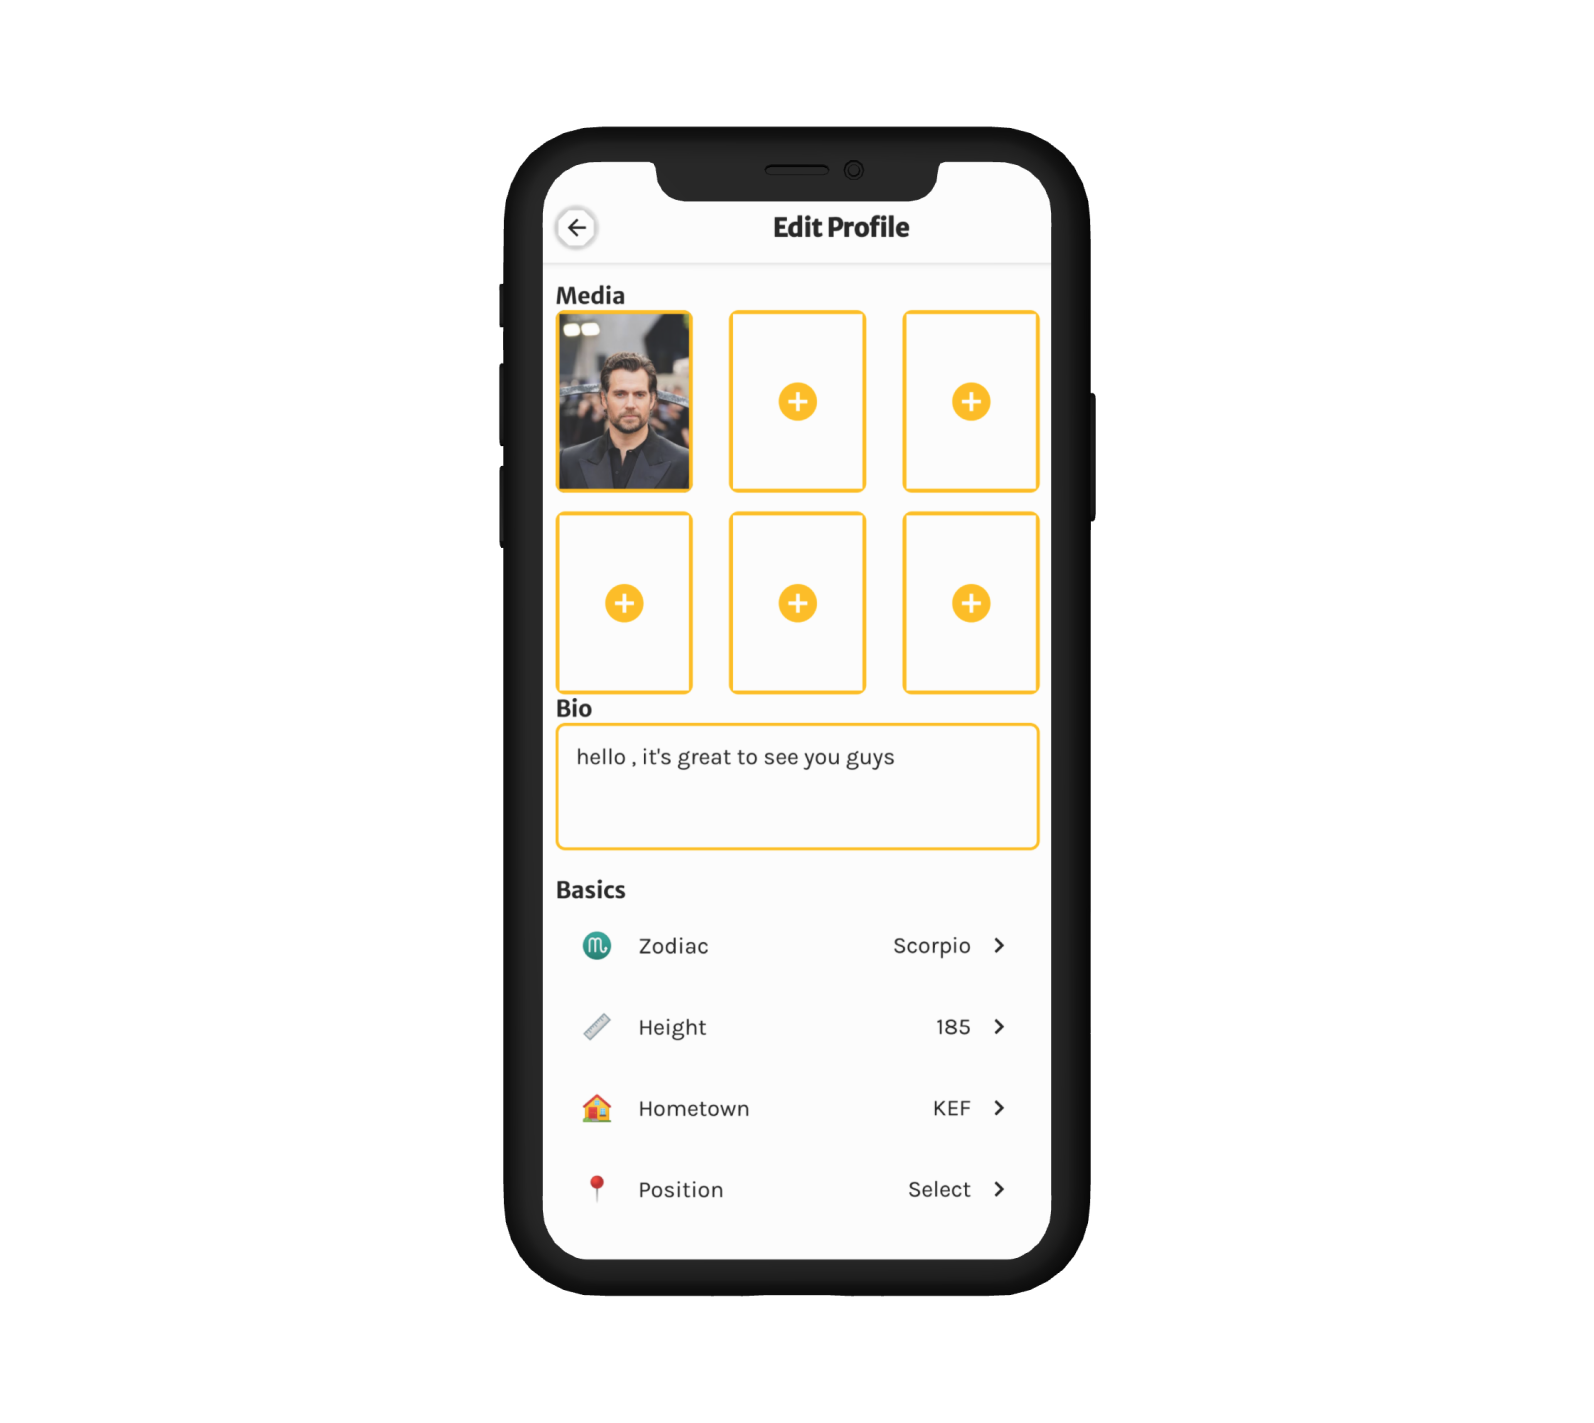
\includegraphics[scale=0.2]{profile managment UI.png}
            \caption{profile management UI} 
            \label{fig: profile management UI}
\end{figure}
\subsection{Password restoration}
Suppose the user has forgotten his password, this will be an inconvenience as he will no longer be able to log in, so we provide a password restoration process so that the user can recover his password safely, first, he types his email, then he checks his mailbox to find a 4-digit code that he can put into the application to finally change his password.
The figure below shows the steps involved in restoring a password.
\begin{figure}[H] 
            \centering
            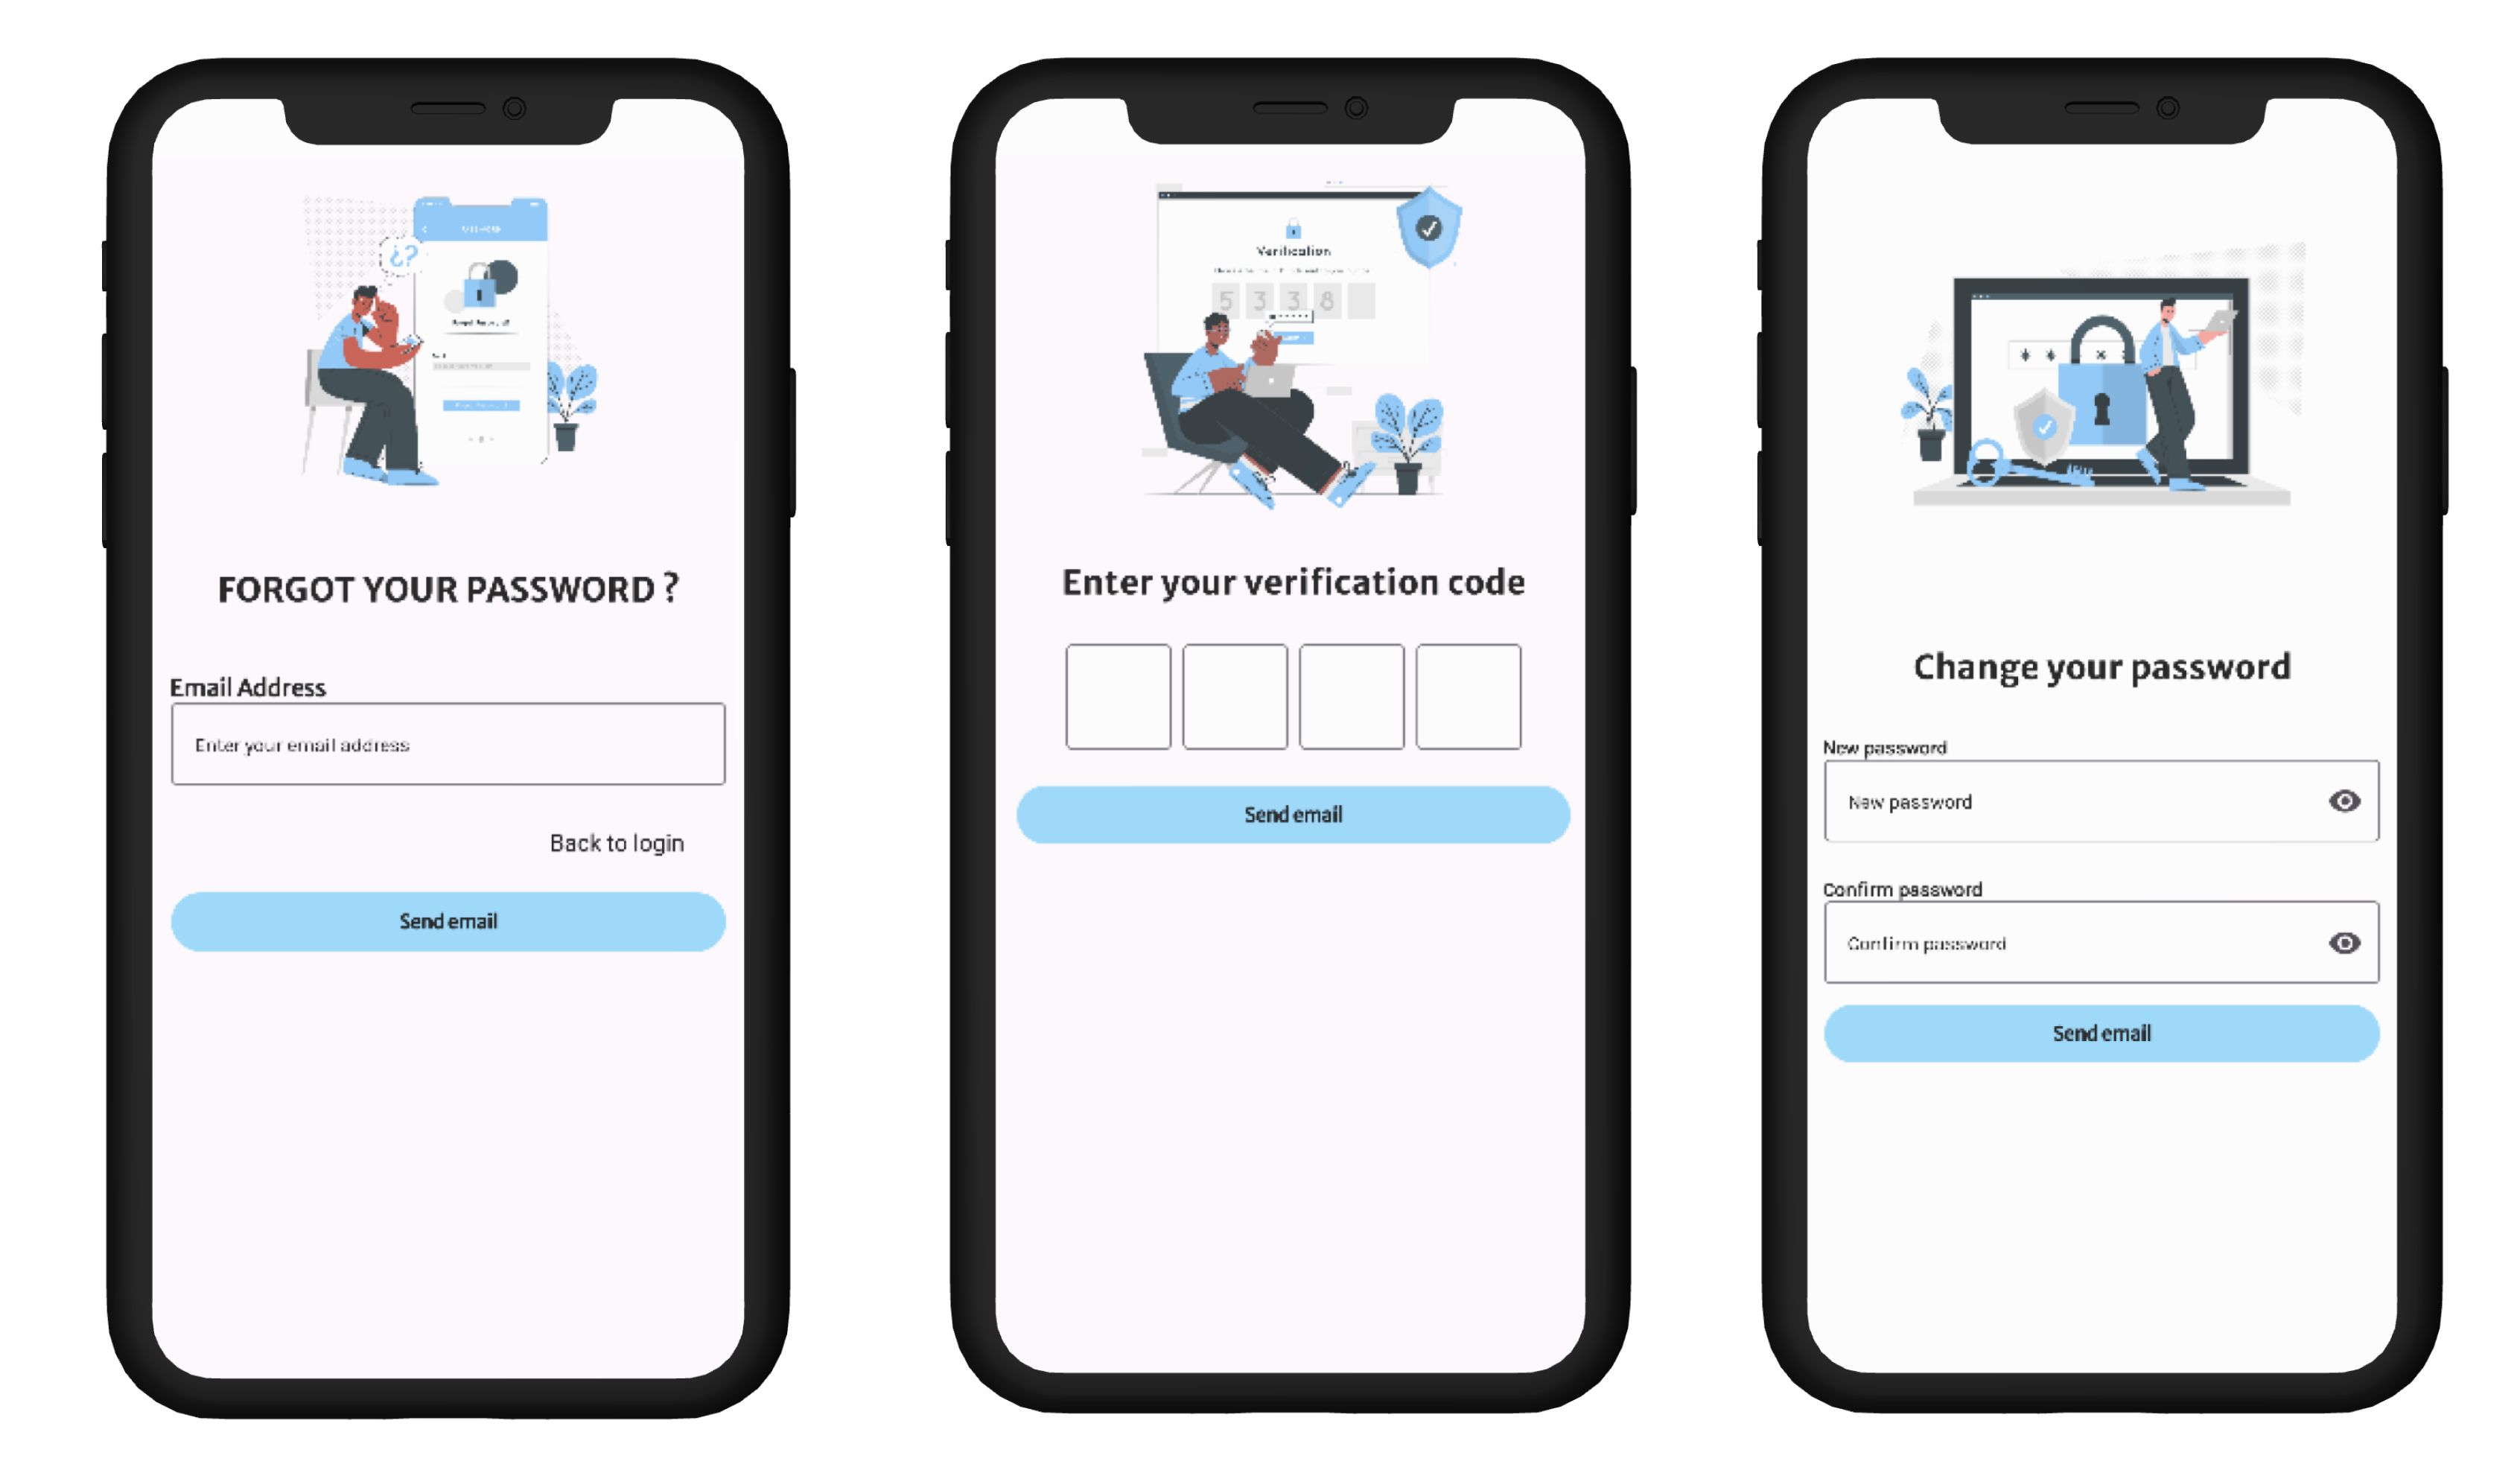
\includegraphics[scale=0.2]{forget password signup.png}
            \caption{forget password UI} 
            \label{fig: forget password UI}
\end{figure}
\section*{Conclusion}
\addcontentsline{toc}{section}{Conclusion}
Sticking to the tradition of the chosen methodology, the first sprint introduced a design of the features that are complete for managing users and their authentication. The fact that it is possible to test and specifically these features in the subsequent sprints is the point that brings the team closer to the goal and the great immersive experience. 

